% ==============================================================
% File     : chapters/00-Introduction.tex
% Date     : 03 Apr. 2022
% Revision : 30 July 2022
% Creator  : Marco Peressutti
% ==============================================================

\chapter{Introduction}
\minitoc

\section{Definition of an Agent}
\begin{itemize}
\item an agent has \side{independent behaviour}: when there is no possibility for direct supervision
\item agents \side{collaborate} and \side{communicate} with each other
\item agents have \side{proactive behaviour}: they have the reasoning possibility to proactively propose some solutions
\item \side{privacy ensurance}: privacy should be ensured via \side{personalization}. A person's interest should not be disclose to some external entity other than the agent itself.
\end{itemize}

\subsection{Formal definitions}
\begin{enumerate}
\item American Heritage Dictionary:

\say{One that acts or has the power or authority to \textbf{act} ... or \textbf{represent} another}

Agents are not independent entities that operate by their own view but they always represent some interest of those who create them.
\item Negroponte

\say{Digital sister in law}

Agents should have specialized expertise and knowledge of preferences of those who create them
\item Russel and Norvig

\say{An agent is anything that can be viewed as perceiving its environment through sensors and acting upon that environment through effectors.}
\item Pattie Maes

\say{Autonomous Agents are computational systems that \textbf{inhabit} some complex dynamic environment, \textbf{sense} and \textbf{act} autonomously in this environment, and by doing so \textbf{realize} a set of goals or tasks for which they are designed}

Agents leave in an environment.
\item IBM

\say{Intelligent agents are software entities that carry out some set of \textbf{operations on behalf of} a user or another program with some degree of \textbf{independence} or \textbf{autonomy}, and in doing so, employ some \textbf{knowledge} or \textbf{representations} of the user’s \textbf{goals} or \textbf{desires}}
\item Coen

\say{Software agents are programs that engage in dialog [and] \textbf{negotiate} and \textbf{coordinate} transfer of information}

Agents must have the possibility to communicate and consequently coordinate and negotiate with one another.
\end{enumerate}

\subsection{Logicale behind autonomous systems}
\begin{itemize}
\item More and more everyday tasks are computer based
\item The world is in a midst of an information revolution
\item Increasingly more users are untrained
\item \side{Lack of programming paradigm} for decentralized program/system construction in dynamic environment.

Existing paradigms were constructed for closed world (i.e. completely specified environment).\\
However in AI the environment is not specified completely (hence there is the need for dynamic exploration of the environment).
\end{itemize}

The solution to this lack of paradigm is to \side{emulate human behaviour}, therefore agents must be able to:
\begin{itemize}
\item perceive the environment
\item affect the environment or act in the environment
\item have a \side{model of behaviour}
\item have intentions/motivations to be fulfilled by implementing corresponding goals.\\
In fact, goals are not enough, the system needs to generate new goals from its intentions and beliefs.
\item communication
\end{itemize}

\subsection{Agent definition and properties}
Wooldridge, Jennings (\side{weak notion}):\\
\say{Agent is a hardware or (more usually) software-based computer system that enjoys the following properties:}
\begin{itemize}
\item \side{autonomy}.\\
Agents operate without the direct intervention of humans or others, and have some kind of control over their actions and internal state.

Hence in order for an agent to be autonomous it must:
\begin{itemize}
\item Act independently
\item Have control over its internal state.

Contrary to objects, agents need to encapsulate behaviour other than their state in the environment.\\
They, in fact, differs from objects since they are required to have a:
\begin{enumerate}
\item \side{degree of autonomy}: agents embody a stronger notion of autonomy than objects, in particular, agents decide for themselves whether or not to perform an action.
\item \side{degree of smartness}: capable of flexible (reactive, pro-active, social) behaviour; standard object models do not have such behaviour
\item \side{degree of activeness}: a multi-agent system is inherently multi-threaded in that each agent is assumed to have at least one thread of active control.
\end{enumerate}
\end{itemize}
\item \side{pro-activeness}.\\
Agents do not simply act in response to their environment, they are able to exhibit goal-directed behavior by taking the initiative.\\
In short, agents must be able to create goals on their own initiative.
\item \side{reactivity}.\\
Agents perceive their environment and respond in a timely fashion to changes that occur in it.\\
In short, communication with the environment.
\item \side{social ability}.\\
Agents interact with other agents (and possibly humans) via some kind of agent-communication language.\\
In short, communication with other agents
\end{itemize}


Wooldridge, Jennings (\side{strong notion}):\\
\begin{itemize}
\item \side{Mentalistic notions}, such as beliefs and intentions are often referred to as properties of strong agents
\item \side{Veracity}, agents will not knowingly communicate false information
\item \side{Benevolence}: agents do not have conflicting goals and always try to do what is asked of it
\item \side{Rationality}: an agent will act in order to achieve its goals and will not act in such a way as to prevent its goals being achieved
\item \side{Mobility}: the ability of an agent to move around a network
\end{itemize}

In addition to these basic properties several other alternatives have been proposed over the years:
\begin{enumerate}
\item Isaac Asimov's laws of robotics:
\begin{enumerate}[label={Law}]
\item One\\
A robot may not injure a human being or, through inaction, allow a human being to come to harm
\item Two\\
A robot must obey orders given to it by human beings except where such orders would conflict with the First Law
\item Three\\
A robot must protect its own existence, as long as such protection does not conflict with the First or Second Law
\item Zeroth\\
A robot may not harm humanity, or, by inaction, allow humanity to come to harm
\end{enumerate}
\item A robot must establish its identity as a robot in all cases
\item A robot must know it is a robot
\item A robot must reproduce. As long as such reproduction does not contradict with Laws 1,2 and 3
\item All robots endowed with comparable human reason and conscience should act towards one another in a spirit of brotherhood
\end{enumerate}

\vfill
Summary:
\begin{itemize}
\item Agents acts on behalf of other entities
\item Agents must have weak agent characteristics
\item Agents may have strong agent characteristics
\end{itemize}

\section{Individual and Group Perspective}
There are two fundamental agents dimensions:
\begin{itemize}
\item \side{Individual agents perspective}. That deals with how to  build agents that are capable of independent autonomous actions in order to successfully carry out the tasks that we delegate to them (\side{Micro aspects}).
\item \side{Group agents perspective}. That deals with how to build agents that are capable of interacting (cooperating, coordinating, negotiating) with other agents in order to successfully carry out the tasks we delegate to them (\side{Macro aspects}).
\end{itemize}

\section{Distributed AI and MAS}
\begin{itemize}
\item Distributed AI is a topic/subject rather than the creation of a brain that is distributed.
\item It became part of AI when it was possible to execute on more than one CPU.
\item For this reason, it is often considered as the intersection of \side{Distributed Computing} and \side{Artificial Intelligence}.

\begin{figure}[!h]
\centering
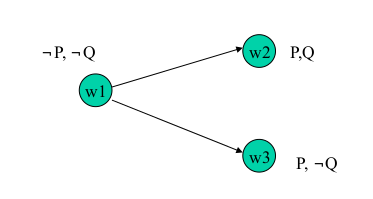
\includegraphics[width=.5\textwidth]{00/00}
\end{figure}

\item Distributed AI includes two different sub field: \side{Distributed Problem Solving (DPS)} and \side{Multi-Agent Systems (MAS)}.
\item DAI deals with several aspects and dimensions such as:
\begin{itemize}
\item Agent granularity
\item Heterogeneity of agents
\item Communication possibilities
\item Methods of distributing control among agents
\end{itemize}
\end{itemize}


\subsection{Distributed Problem Solving (DPS)}
DPS considers how the task of solving a particular problem can be divided among a number of modules that cooperate in dividing and sharing knowledge about the problem and its evolving solution(s):
\begin{itemize}
\item In pure DPS systems, all interaction strategies are incorporated as an integral part of the system
\item DPS has focused on achieving goals under varying environmental conditions, having agents with established properties
\end{itemize}

In other terms in DPS:
\begin{enumerate}
\item a problem is divided into modules 
\item each module is allocated to a different agent
\item the agents will solve the problem by means of communicating the solution to their allocated module
\end{enumerate}

\subsection{Multi-Agent Systems (MAS)}
\begin{itemize}
\item MAS are designed in a decentralized way with great part of independency and autonomy
\item Agents with individual preferences will interact in particular environments such that each will consent to act in a way that leads to desired global goal
\item MAS asks how, for a particular environment, can certain collective goal be realized if the properties of agents can vary uncontrollably:
\begin{itemize}
\item loosely-coupled networks of problem solvers (agents) that work together to solve problems that are beyond their capabilities
\item no necessary guarantees about other agent
\end{itemize}
\item MAS contain a number of agents which interact with one another through communication. The agents are able to act in an environment; where each agent will act upon or influence different parts of the environment. If two field of influence overlap, the conflict is (hopefully) resolved via negotiation and communication

\begin{figure}[!h]
\centering
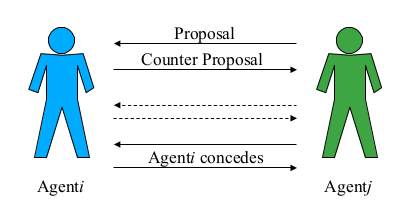
\includegraphics[width=.9\textwidth]{00/01}
\end{figure}

\item An important concept in MAS is that there is no central control (because the control is distributed to the various agents) and knowledge or information sources may also be distributed
\end{itemize}

In other terms, contrary to DPS, MAS do not deal with task to be solved but rather rules to be followed, and these rules are for example, their beliefs, desire and intentions or protocols for negotiation and communication.

The motives behind the use of MAS are:
\begin{itemize}
\item To solve problems that are too large for a centralized agent
\item To allow interconnection and inter-operation of multiple legacy systems
\item To provide a solution to inherently distributed problems
\item To provide solutions which draw from distributed information sources
\item To provide solutions where expertise is distributed
\item To offer conceptual clarity and simplicity of design
\end{itemize}

The are two sub-classes of MAS:
\begin{itemize}
\item \side{Cooperative}.

Agents are designed by interdependent designers.\\
Agents act for increased good of the system.\\
Agents are concerned with increasing the performance of the system.\\

Hence if we imagine that the goodness of the system is represented by a global function. Agents in a cooperative MAS will try to maximize such function.
\item \side{Self-interested}

Agents designed by independent designers.\\
Agents have their own agenda and motivation.\\
Agents are concerned with the benefit and performance of the individual agent.\\

Hence, if we imagine that the goodness of each agent is represented by a local function (one for each agent). They will try to maximize their own function.	
\end{itemize}

Among the benefits of using MAS over DPS we find that, MAS:
\begin{itemize}
\item  Faster problem solving
\item Decrease in communication
\item  Flexibility
\item Increased reliability
\end{itemize}
However, its main drawback is the \side{lack of predictability}.

\vfill
Summary of definitions:
\begin{itemize}
\item Distributed Computing: focus on low level parallelization and synchronization
\item Distributed AI: Intelligent control as well as data may be distributed. Focus on problem solving, communication and coordination
\item DPS: Task decomposition (task sharing) and/or solution synthesis (result sharing): information management
\item MAS: Behavior coordination and management
\end{itemize}
\newpage

\section{Emergence, Swarm Intelligence and other terms}
\subsection{Emergence}
With the term \side{Emergence}, we refer to those global (macro level) behaviour, patterns and properties that arise from the interactions between local parts of the system (micro level).\\
Systems that exhibit emergence can be characterized as simple, robust and adaptive.
\subsection{Swarm Intelligence}

The term \side{Swarm Intelligence} refers to any attempt to design algorithms or distributed problem-solving devices inspired by the collective behaviour of social insect colonies and other animal societies.\\
Multi-robot systems, which implement or adapt the concept of emergent behaviour, are commonly referred to as \side{swarm robotic systems}.
\subsection{Self-Organisation}
\phantom{c}\side{Self-Organization} is a dynamical and adaptive process where systems acquire and maintain structure themselves, without external control.\\
The term self-organization is also used as the process that leads to the state of emergence.\\
Self-organization and emergent systems are distinct concepts, they still have one thing in common, that is: there is no explicitly external control whatsoever.\\
The main difference between self-organization and emergence is that in the case of self-organization, individual entities can be aware of the system's intended global behaviour. In consequence, self-organization can be seen as a weak form of emergence.\\
The intuitive and regularly used approach to realize self-organization is applying the concept of feedback loops.

\subsection{Self-Adaptation}
When the approach with feedback loop is applicable to single entity system it is usually referred as \side{self-adaptation}.\\
Self-adaptive software modifies its own behaviour in response to changes in its operating environment.\\
If a decentralized system containing several entities exhibits adaptive behaviour to external changes this is as well considered self-adaptation.

\subsection{Characteristics of Emergence, Swarm Intelligence, Self-Adaptation and Self-Organization}
Having ensembles of robust (multi-)agent systems that maintain their structure and feature a high level of adaptation.\\
It would no longer be necessary to exactly specify the low lever system behaviour in all possible situations that might occur, but rather leaving the system with a certain degree of freedom to allow for autonomous reaction and adaptation to new situations in an intelligent way.

\subsection{Application}
Self-organization algorithms have been applied in many multi-agent domains, like combinatorial optimization, communication networks and robotics.\\
The algorithms, respectively mechanism, are used for various purposes, like motion control, information sharing and decision making.
